%!TEX root = ../main.tex
% -*- root: ../main.tex -*-
\section{Implementation}\label{sec:implementation}

%As previously stated, in this paper we also present working prototypes of domain-side and client-side middlewares. In particular, the former consist of a mobile domain and a local-edge domain, while the latter consists of a Android mobile client device. 

To demonstrate the feasibility of A3-E in managing the life-cycle of continuum applications, we describe the implementation of A3-E. Due to its complexness, we focus on the implementation of the self-management loop for handling Allocation from both provider and client viewpoints. 

\subsection{Control Theory-based $\mu$-Service Allocation}~\label{sec:ps_allocation}

To cope with the low-latency requirement of continuum applications and a highly dynamic workload  (e.g., from users that quickly enter and leave a particular edge area) we 
%TODO move to the problem formulation i) consider the \textit{response time} as the reference metric of QoS and ii) 
propose a fast and scalable materialization of the provider-side self-management loop based on control theory. In literature one can find many approaches of dynamic resource allocation based on heuristics~\cite{dustdar0}, artificial intelligence~\cite{ia1} and queue theory~\cite{queue1}. Nevertheless, we adopted an extremely lightweight control theoretical technique to fully exploit the container technology~\cite{Quatrocchi2016discrete}: compared to virtual machines containers can be booted in few seconds, therefore we used controllers that are able to change the resource allocation with a very fast period (i.e., in the order of few seconds).

Figure~\ref{fig:A3Edomain-manager} depicts an overview of the control system, which is responsible for the deployment of containers to the cluster of (virtual) machines composing a domain's pool of resources (or the \textit{plant} in control-theoretical terms). Each container provides the runtime environment required for the execution of a given continuum $\mu$-service; and multiple instances of $\mu$-services may coexist in one or more machines (horizontal scalability).

\begin{figure}[tbp]
	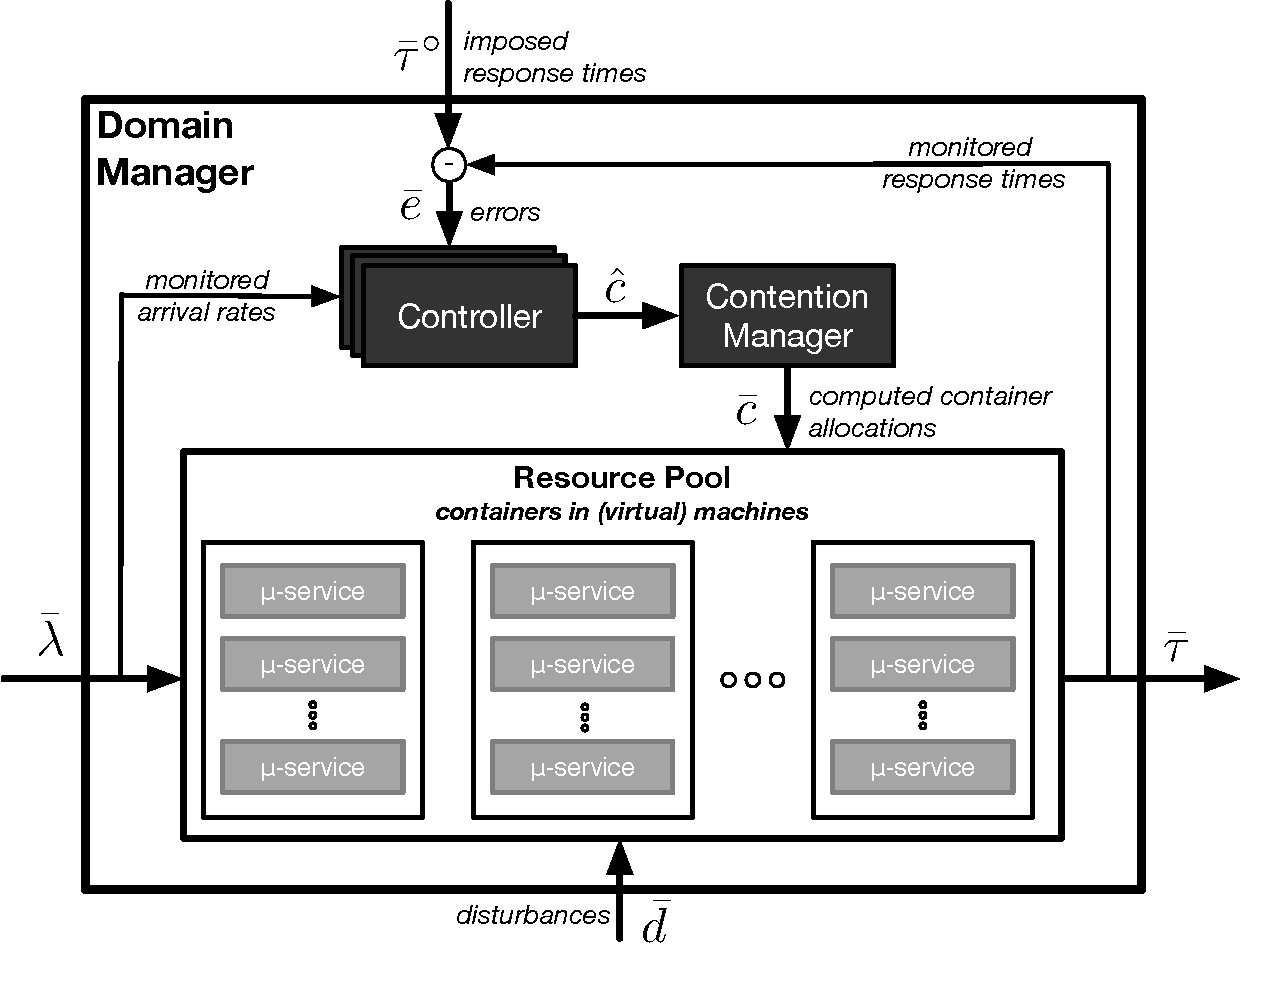
\includegraphics[width=0.65\textwidth]{figs/domain-manager-allocation}
	\caption{Control loop implementing the self-management of a domain's resources}
	\label{fig:A3Edomain-manager}
\end{figure}

%The system 
%to be controlled, or the \textit{plant} in control-theoretical terms, is the provider's resource %pool composed by a cluster of (virtual) machines. 

%Containers are deployed in those machines and they execute $\mu$-services. Each service can be replicated on different machines, enabling horizontal scalability. 

The control plant is subject to different signals that could be measurable (input variables) or unknown (disturbances). Considering a discrete time, for each $\mu$-services $s_j \in S$ we define $\lambda_j(k)$ as the function of the measured arrival rate of requests at each control time $t$.
; while $\bar{\lambda}(k)$ is the corresponding vector for all $s_i \in S$. 
%TODO c(k) is the same as f_{i,j}(k) and \bar{c}(k) is the same as  F_{i}. 
At time $t$ each $\mu$-service $s_j \in S$ is executed in a $c_j(k)$ number of allocated containers.%, while $\bar{c}(k)$ is the corresponding vector for all $s_i \in S$. 
The disturbances are defined as $\bar{d}$ and cannot be directly controlled and measured by definition. Finally, $\bar{\tau}$ is the system output and corresponds to the vector of response times of each $\mu$-service; while $\bar{\tau}^\circ$ corresponds to the vector of desired response times or control set-point (according to the SLA of each $\mu$-service). 

In our current setup the function $\bar{\tau}^\circ(k)$ does not vary over time, meaning a constant QoS for each  $\mu$-service. Of course, these values should be set below the thresholds defined in the SLA (i.e., $\forall\ k \in \mathbb{N} \wedge  s_j \in S, {\tau}^\circ_j(k) \le \Delta_j$). Moreover, since response time cannot be measured instantaneously but by aggregating the execution times of different requests over a predefined time window, many aggregation functions could be used without any change to the system model and controller. For example in our current setup we are using the $99th$ percentile function. 

We dedicate one controller per $\mu$-service with the goal to compute the next container allocation in order to obtain:
{\scriptsize
\begin{equation}
\tau_j(k)^\circ - \tau_j(k) = e_j(k) = 0\quad \forall{k} \ge 0
\end{equation}
}%
or more realistically, considering all the services:
{\scriptsize
\begin{equation}
\bar{e}_j(k) \simeq 0 \quad \forall{k} \ge 0
\end{equation}
}%
To do that the controllers must model the system 
%with enough details to govern the dynamics of the plant. In control theory this is done 
by defining a characteristic function. We assume that this function does not need to be linear but regular enough to be linearizable in the domain space of interest. Moreover, we consider this function to be dependent on the ratio of the number of allocated containers $c$ and the request rate $\lambda$. This function, $f$ to give it a name, is intuitively monotonically decreasing towards a possible lower horizontal asymptote, as it can be assumed that once the parallelism degree of a $\mu$-service is fulfilled by the available containers, adding new ones causes no further decrease in the response time. More specifically, we found a practically acceptable function to be
{\scriptsize
\begin{equation}
f_j \left( \frac{c_j(k)}{\lambda_j(k)}\right)  = \widetilde{u}_j(k) = c_1+\frac{c_2}{1+c_3\frac{c_j(k)}{\lambda_j(k)}}
\label{eqn:CsysModel-f}
\end{equation}
}%
\noindent where parameters $c_1$, $c_2$, and $c_3$ were obtained through profiling of each $\mu$-service. Thus we obtain the following dynamic system:
{\scriptsize
\begin{equation}
\tau_j(k)  = p_j \tau_j(k-1) + (1-p_j)\widetilde{u}_j(k-1)
\label{eqn:CsysModel-s}
\end{equation}
}%
where $p \in [0,1)$ is the single pole of the system estimated with step response analysis. As control techniques we rely on PI controllers because they are able to effectively control systems dominated by a first order dynamic ~\cite{aastrom1995pid} (i.e., representable with first order differential equations) such as the studied ones. PI controllers compute the next state of a plant by using two contributions: one that is proportional and another that is integral to the error $e$. Algorithmically, $\forall\ k \in \mathbb{N} \wedge  s_j \in S$: 
{\scriptsize
\begin{align*}
\begin{split}
e   &:= \tau_r^{\circ}-\tau_r;\\
x_R &:= x_{R_p}+(1-p)*e_p;\\
c   &:= \lambda*f_{inv}((\alpha-1)/(p-1)*(x_R+e));
\end{split}
\begin{split}
c   &:= max(min(Kmax,c), Kmin);\\
x_{R_p} &:= (p-1)/(\alpha-1)*f(c/\lambda)-e;\\
e_p  &:= e;
\end{split}
\end{align*}
}%
where the ``$p$'' subscript denotes ``previous'' values, i.e., those corresponding to the previous step, while ``$f$'' and ``$f_{inv}$'' correspond to the characteristic function and its inverse, respectively, while $\alpha \in [0,1)$ is the single pole of the controller (the higher the value the faster will be the error convergence to $0$). 

The algorithm is run by each controller at each control step independently (i.e. without synchronization) to compute the next container allocation for the corresponding $\mu$-service. $\hat{c}$ is the vector containing the allocations of all the services. $\hat{c}$ is not immediately actuated (through the container manager of choice such as Docker Swarm~\cite{Swarm} or Kubernetes~\cite{Kubernetes}) since the sum of the allocations could be greater than the entire capacity of the resource pool. In fact $\hat{c}$  is passed to another control component called  \textit{ContentionManager}. The  output of ContentionManager is a vector $\bar{c}$, the actual container allocations of $\mu$-services, defined as 
\begin{equation}
\bar{c}(k) =
\begin{cases}
\hat{c}(k),& \text{if \textit{no resource contention}}\\
scaleDown(\hat{c}(k)),              & \text{otherwise}
\end{cases}
\label{eqn:CsysModel-SS}
\end{equation} 
where function $scaleDown$ scales down the allocations to be equal to the maximum capacity according to a priority policy. 

As an example, in the scenario introduced in Section~\ref{sub:example}, critical applications should have a higher priority with respect to applications such as the AR for tourists~\cite{GarrigaMendonca2017}. In case of contention, edge-based $\mu$-services might become unavailable (or available with an higher response time) to the AR applications. In that case the AR and other low-priority applications could have to rely on $\mu$-services from their mobile domain or a cloud provider domain. Finally \textit{ContentionManager} updates the state of each controller (variable $x_{R_p}$) to reflect the actual allocation.

\subsection{Multi-Attribute Domain Selection}~\label{sec:cs_allocation}

%As described in Section~\ref{sec:proposal}, the CSM component interacts with DSM from different domains that could be either discoverable using a DNS-like mechanism or advertisement. 

The main goal of the client-side middleware\footnote{Documentation and source code are available at \url{https://github.com/deib-polimi/A3-E-CSM}} is to allow client applications to invoke continuum $\mu$-services without knowing where they will actually be executed within the computing continuum.
%: locally on the mobile domain, in a local-edge server, in a mobile-edge server, or in the cloud. 
Its \textit{domain selection} algorithm consists of a multi-attribute function that takes into account the measured QoS and the requirements. %The provided implementation targets Android-based devices. However, it does not use Android-specific technology and can therefore be generalized to other mobile platforms. 

The provided implementation consists of components responsible for Awareness, the Acquisition, and finally the set of  components responsible for Allocation, during which domain selection occurs (see Sec.~\ref{sec:A3-E-allocation}). The latter implement a self-managing loop that: (i) monitors $\mu$-services provided by different domains in terms of QoS metrics; (ii) analyzes the best alternative satisfying requirements of the client application; and (iii) updates the domain selection for a given $\mu$-service. 

In addition to A3-E's \textit{Location requirements}, the prototype considered two types of \textit{QoS requirements}:

\begin{enumerate}
	
	%	\item \textit{Location Requirement}s constrain where the microservice can be placed within the continuum, i.e., \textit{LOCAL}, \textit{LOCAL\_EDGE}, \textit{MOBILE\_EDGE}, or \textit{CLOUD} or a combination of the above; 
	
	\item a \textit{Latency Requirement} constrains network latency, i.e., \textit{ANY}, \textit{LOW} or \textit{VERY\_LOW}; and 
	
	\item a \textit{Computational Requirement} defines how relevant it is for a $\mu$-servi to have fast computing, i.e., \textit{ANY}, \textit{FAST} or \textit{VERY\_ FAST}. 
\end{enumerate}

The latter is defined as a fixed score ranging from $1$ to $5$\footnote{Labeling computational power is also common in the cloud where different tiers of virtual machines are available -- \url{https://aws.amazon.com/ec2/instance-types/}}. By default, the local domain has a score of $1$, the edge domains have a score of $4$, while the cloud domains have a score of $5$. Note that since the cloud provides the illusion of infinite scalability it gets the maximum score, regardless of the VMs that are actually being used. More sophisticated approaches with dynamic scores taking into account the saturation of the domain or the device's battery level (in the case of a mobile domain) are considered as future work.

\begin{algorithm}[thb]
	\caption{A3E Selection Algorithm}
	\label{alg:selection}
	\begin{algorithmic}[1]
		
		\Function{selectDomain}{A3EService $microservice$, A3EDomain[] $identifiedDomains$}
		\State$scoreRange \gets 5$
		\State $maxLatency \gets \Call{computeMaximumLatency}{identifiedDomains}$
		\State $maxCpuPower \gets \Call{computeMaximumComputationalPower}{identifiedDomains}$
		\State $latencyWeight \gets microservice.getLatencyRequirement()$ 
		\State $cpuPowerWeight \gets microservice.getComputationalPowerRequirement()$ 
		\State $maxScore \gets 0$
		\State $selectedDomain \gets null$
		\ForAll{$domain \in identifiedDomains$ } 
		\State $latency \gets domain.getLatency()$ 
		\State $cpuPower \gets microservice.getComputationalPower()$ 
		\State $latencyScore \gets latencyWeight*((scoreRange-1)*(1 - latency/maxLatency)+1)$ 
		\State $cpuPowerScore \gets cpuPowerWeight*(scoreRange*(cpuPower/maxCpuPower))$
		\State $score \gets (latencyScore + cpuPowerScore) / (latencyWeight + cpuPowerWeight)$
		\If{$score \geq maxScore$} 
		\State $maxScore \gets score$
		\State $selectedDomain \gets domain$
		\EndIf
		\EndFor 
		\State \Return $selectedDomain$
		\EndFunction
	\end{algorithmic}
\end{algorithm}

%TODO [Danilo] improve this paragraph
Algorithm~\ref{alg:selection} describes the procedure employed in the microservice selection. The algorithm computes a score ranging from $0$ to $5$ (line $2$). First, it retrieves the maximum computational power and network latency from available domains (line $3$ and $4$). Then, it retrieves the weights assigned to each QoS metric (lines $5$ and $6$). These weights correspond to the values associated to the \textit{LatencyRequirement} and \textit{ComputationalRequirement} of the microservice. The \textit{ANY} value corresponds to a weight of $0$, a latency requirement of \textit{LOW} and a computational power requirement of \textit{FAST} correspond to a weight equal to $1$, while a latency requirement of \textit{VERY\_LOW} and a computational power requirement of \textit{VERY\_FAST} correspond to a weight equal to $2$. 

For each domain, the algorithm computes the overall score (line $9$ to $14$). The latency score is computed by normalizing the value retrieved at line $10$ with the maximum latency previously computed. The normalized value ranges from $0$ to $1$, the higher this value is the higher the latency. Since a higher score should mean lower latencies, the algorithm computes the complement of this value and adds $1$ to avoid scores equal to $0$. The latency score is computed to be between $1$ and $5$, and multiplied by the microservice's latency weight (line $12$). The computational power score is computed by normalizing the domain computational power retrieved at line $11$ with the maximum value across the identified domains. Again, the score for this metric is computed to be between $1$ to $5$ and multiplied by its weight (line $13$). Finally, the overall score is the weighted average between the scores obtained by the domains for the two QoS metrics.

%Two considerations must be added for this algorithm. First, 
Algorithm~\ref{alg:selection} is an instantiation of the SMART decision process~\cite{Olson1996}, in which multiple competing QoS attributes are taken into account using the following formula:

\begin{equation}
Smart(c) = \frac{\sum_{i=1}^{n} QoSAtrribute_i(c)*weight_i}{\sum_{i=1}^{n}weight_i} \label{eq:smart}
\end{equation}

\noindent
where $c$ is a domain, the QoS attributes values are network latency and the computational processing time (thus $n$ is $2$), and their weights are represented by the aforementioned latency and computation requirements. Note that, when available, \textit{edge domains have the highest chances of being selected}, since they usually combine a low network latency and a medium-to-high computational power. Finally, each microservice is mapped to the domain that best satisfies its requirements.

%Last but not least, during the \textit{Engagement} phase the CSM handles C-requests triggered by the client application for a specific microservice in the continuum and invokes the domain previously selected. Domains are bound to an invocation resolver: edge and cloud domains resolvers fire an HTTP request, while the resolver bound to a mobile domain will broadcast an Android event containing the request along with a callback. In particular, this broadcast is handled by the mobile domain manager.